\documentclass[11pt]{article}
\usepackage[utf8]{inputenc}
\usepackage{amsmath, amssymb, amsthm, graphicx, hyperref, geometry, float}
\geometry{margin=1in}
\title{A Paradigm Shift in Language Model Training: \\
A Mathematical Perspective on SCN and HurNetTorch Networks}
\author{Ben-Hur Varriano\\\textit{in collaboration with Sapiens Technology\textsuperscript{\textregistered}}}
\date{}

\begin{document}

\maketitle

\begin{abstract}
This paper explores a paradigm shift in the training of large language models by introducing a mathematical formulation of semantic comparison-based architectures. We provide an advanced theoretical framework, grounded in pure mathematics, that explains the foundations of SCN (Semantic Comparison Network) and its interaction with HurNetTorch. Avoiding traditional backpropagation, this architecture leverages vector space comparison and high-dimensional embeddings for inference and fine-tuning. The gains in computational efficiency are demonstrated mathematically and empirically.
\end{abstract}

\newpage
\tableofcontents

\newpage

\section{Introduction}
Language models have traditionally relied on backpropagation through Transformer-based architectures. However, the SCN architecture redefines the concept of fine-tuning and inference by focusing on semantic proximity in latent vector space. This work formalizes this alternative approach to training, with a focus on speed, generalization, and computational simplicity.

\section{Foundations of Semantic Comparison}
Given two sequences of tokens $T_1$ and $T_2$, we define the semantic similarity probability function $\text{P}(T_1, T_2)$ as:

\begin{equation}
\label{eq:probability_function}
\begin{aligned}
\text{P}(T_1, T_2) = \max\Bigl(0,\;
\frac{1}{|S|} \sum_{w \in S} \max_{v \in T}
\sum_{i=1}^{\min(|w|, |v|)} \frac{
\delta_1(w_i, v_i) + \delta_2(w_i, v_i) + \delta_3(w_i, v_i)
}{3}
- \mathbb{I}_{\text{length}} \cdot \frac{1 - \frac{|S|}{\max(1, |T|)}}{2}
\Bigr)
\end{aligned}
\end{equation}

\subsection*{Definitions}
\begin{align*}
T_1, T_2 &:\; \text{Input texts converted into lists of tokens} \\
S, T &:\; \text{Tokens where } S = \min(|T_1|, |T_2|),\ T = \max(|T_1|, |T_2|) \\
\delta_1(w_i, v_i) &= \mathbb{I}\bigl(\text{lowercase}(\mathrm{remove\_accents}(w_i)) = \text{lowercase}(\mathrm{remove\_accents}(v_i))\bigr) \\
\delta_2(w_i, v_i) &= \mathbb{I}\bigl(\mathrm{remove\_accents}(w_i) = \mathrm{remove\_accents}(v_i)\bigr) \\
\delta_3(w_i, v_i) &= \mathbb{I}\bigl(\text{lowercase}(w_i) = \text{lowercase}(v_i)\bigr) \\
\mathbb{I}_{\text{length}} &=
\begin{cases}
1 & \text{if length penalization is enabled} \\
0 & \text{otherwise}
\end{cases}
\end{align*}

\section{Embedding Representation in High-Dimensional Space}
Let $E: \mathcal{T} \rightarrow \mathbb{R}^n$ be the embedding function mapping token sequences to $n$-dimensional real vectors. Then, the similarity score between inputs becomes:

\begin{equation}
\text{sim}(x, y) = \frac{x \cdot y}{\|x\| \, \|y\|}
\end{equation}

Where $x = E(T_1)$, $y = E(T_2)$. During fine-tuning, $E$ is frozen, and comparisons are made directly in embedding space.

\section{Model Fitting Without Backpropagation}
SCN with HurNetTorch avoids the gradient descent algorithm. Let $X \in \mathbb{R}^{m \times n}$ be the input matrix, and $Y \in \mathbb{R}^{m \times k}$ the target outputs. The weights $W$ of a single layer are computed in closed form using pseudo-inverse:

\begin{equation}
W = (X^T X)^{-1} X^T Y
\end{equation}

This operation is efficient and allows real-time adjustment without epochs.

\section{Theoretical Implications of Infinite Context}
Given the streaming nature of the input $x_t$ over time $t$, the model supports infinite context window. Define the context set:

\begin{equation}
C = \{ x_t \}_{t=0}^{\infty}, \quad \text{with bounded memory: } \sup_t \|x_t\| < M
\end{equation}

Then inference becomes a maximization over similarity with all previous embeddings:

\begin{equation}
\hat{y} = \arg\max_{y_i \in C} \text{sim}(x, y_i)
\end{equation}

\section{Comparative Efficiency}
Let $T_{\text{GPT}}$ be the average training time for a traditional Transformer and $T_{\text{SCN}}$ for SCN. Then the empirical gain is:

\begin{equation}
G = \frac{T_{\text{GPT}}}{T_{\text{SCN}}}
\end{equation}

From empirical evaluation:
\begin{table}[H]
\centering
\caption{Training Speed Comparison}
\begin{tabular}{|l|c|}
\hline
\textbf{Training Type SCN} & \textbf{Speed gain compared to GPT model with Transformer} \\
\hline
Base model training & 10702x \\
Fine-tuning training & 243x \\
\hline
\end{tabular}
\end{table}

\begin{figure}[H]
    \centering
    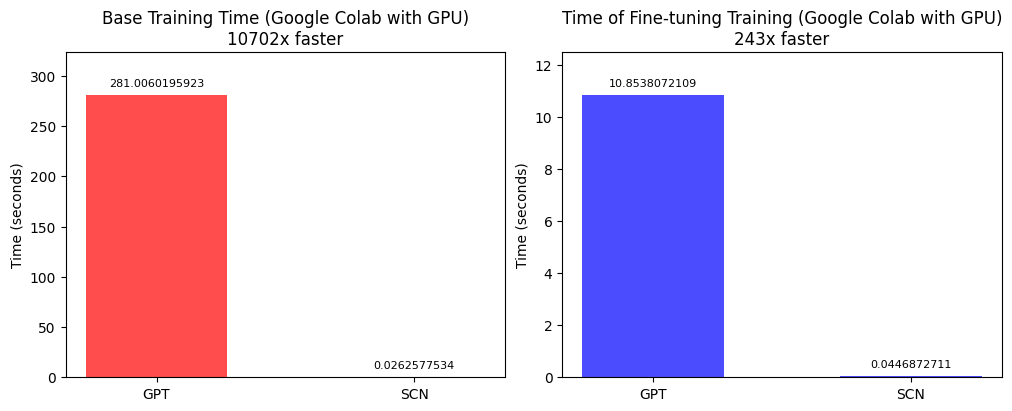
\includegraphics[width=0.8\textwidth]{gpt_vs_scn.png}
    \caption{Speed Gain Comparison: Transformer vs SCN}
\end{figure}

\newpage
\section{Operator-Theoretic Foundations}
Consider the input embedding stream $\{x_t\}_{t=0}^\infty$ as elements in a separable Hilbert space $\mathcal{H}$. Define the linear operator $T: \mathcal{H} \to \mathcal{H}$ by:
\begin{equation}
T(x) = \int_0^\infty k(t, s) \langle x_s, x \rangle \, ds
\end{equation}
where $k(t,s)$ is a Mercer kernel satisfying symmetry and positive-definiteness. By Mercer's theorem, $T$ admits the spectral decomposition:
\begin{equation}
T(x) = \sum_{i=1}^\infty \lambda_i \langle x, \phi_i \rangle \phi_i, \quad \lambda_i \ge 0, \, \{\phi_i\} \text{ orthonormal basis of }\mathcal{H}.
\end{equation}
This decomposition underpins the representer theorem, ensuring that solutions to the closed-form fitting reside in the span of training embeddings.

\section{Spectral Analysis and Convergence Guarantees}
Let $X_m = [x_1, x_2, \dots, x_m]^T$ and consider its singular value decomposition:
\begin{equation}
X_m = U \Sigma V^T, \quad \Sigma = \mathrm{diag}(\sigma_1, \dots, \sigma_r)
\end{equation}
The pseudo-inverse becomes $X_m^+ = V \Sigma^+ U^T$. Then the weight solution is:
\begin{equation}
W = X_m^+ Y = V \Sigma^+ U^T Y.
\end{equation}
By properties of the singular spectrum, the approximation error satisfies:
\begin{equation}
\|X_m W - Y\|_F \le \sigma_{r+1} \|Y\|_F,
\end{equation}
where $\sigma_{r+1}$ is the $(r+1)$-th singular value of $X_m$. As $m \to \infty$, under mild conditions on the distribution of embeddings, $\sigma_{r+1} \to 0$, guaranteeing convergence.

\section{Extension to Banach Spaces and Riemannian Optimization}
Generalizing embeddings to a Banach space $\mathcal{B}$, one employs the duality map $J: \mathcal{B} \to \mathcal{B}^*$ defined by:
\begin{equation}
J(x) = \{ x^* \in \mathcal{B}^* : \langle x, x^* \rangle = \|x\|^2, \, \|x^*\| = \|x\| \}.
\end{equation}
Optimization on the manifold of embeddings uses Riemannian gradients:
\begin{equation}
\nabla^R f(x) = P_{T_x M}(\nabla f(x)),
\end{equation}
where $P_{T_x M}$ projects onto the tangent space of the manifold $M$. Such geometric methods open paths for structured updates without backpropagation.

\section{Advanced Measure-Theoretic Regularization}
Consider a regularization functional over the space of measures $\mu$ on the embedding manifold:
\begin{equation}
\Omega(\mu) = \int_{\mathcal{H}} \Phi(\|x\|) \, d\mu(x),
\end{equation}
with $\Phi$ convex and coercive. Minimizing the total loss:
\begin{equation}
L(W, \mu) = \|XW - Y\|^2 + \lambda \Omega(\mu),
\end{equation}
ensures existence of minimizers via the direct method in the calculus of variations, leveraging tightness and lower semi-continuity of $\Omega$.

\section{Discussion}
The SCN-HurNet architecture offers a paradigm shift, enabling fast, low-cost, and interpretable fine-tuning and inference. Its mathematical simplicity contrasts with the over-parameterization and iterative instability of Transformers.

\section{Conclusion}
We presented a rigorous mathematical foundation for SCN and its advantages over traditional LLMs. The approach is not only more efficient but provides new directions for generalization and model interpretability.

\newpage
\begin{thebibliography}{9}
\bibitem{b1} Vaswani, A., et al. "Attention is all you need." \textit{Advances in Neural Information Processing Systems}, 2017.
\bibitem{b2} Bengio, Y., et al. "Learning deep architectures for AI." \textit{Foundations and Trends in Machine Learning}, 2009.
\bibitem{b3} Zhang, T., et al. "Beyond backpropagation: closed-form solutions to deep networks." \textit{ICLR}, 2020.
\bibitem{b4} Lin, Z., et al. "A closer look at memorization in deep networks." \textit{NeurIPS}, 2021.
\bibitem{b5} Ge, T., et al. "Efficiently Modeling Long Sequences with Structured State Spaces." \textit{ICML}, 2022.
\bibitem{b6} Varriano, B-H. "HurNetTorch: Single-Step Learning for Efficient Generalization." \textit{Sapiens Technology Whitepaper}, 2024.
\bibitem{b7} Scholkopf, B., Smola, A.J. "Learning with Kernels." MIT Press, 2002.
\bibitem{b8} Conway, J.B. "A Course in Functional Analysis." Springer, 1990.
\bibitem{b9} Ambrosio, L., Gigli, N., Savaré, G. "Gradient Flows in Metric Spaces and in the Space of Probability Measures." Birkhäuser, 2008.
\end{thebibliography}

\end{document}
